% Owner: W2  |  Budget: ~1.75 columns  |  16 pts
% Sources: results/tables/04_coefficients.md, 05_error_cases.md (I2)
\section{Analysis}
\label{sec:analysis}

\subsection{Coefficients and Statistical Significance}
% Slides p.16 (8%): standardized coefficients with 95% CI, p-value (name the
% test), VIF; check signs against §4; explain reversals; practical significance
% in target units. Slides ask for EVERY feature: Figure (forest plot) shows all 55
% numeric/ordinal predictors; the 159 one-hot columns are summarized in the text
% and listed in full on GitHub. Figure script: figures/plot_coef_forest.py
% CAUTION: after Holm correction no coefficient is significant (min 0.214);
% 29 of 214 have a 95% CI excluding 0 only WITHOUT correction; 159 VIFs are inf.
Figure~\ref{fig:coef} shows every numeric and ordinal predictor of the final model (55 of 214 columns) with its standardized coefficient, bootstrap 95\% CI and $p$-value (1{,}000 training resamples, pipeline fixed), and VIF.
The 159 one-hot columns of the 19 nominal features are small: none exceeds $|\beta| = 0.019$ (poured-concrete foundation), a quarter of QualityArea's.
The seven largest coefficients are all positive; only OverallCond reverses its training correlation ($r = -0.03$).
Older houses carry higher condition ratings ($r = -0.39$ with YearBuilt), so that correlation mixes age with condition; at a fixed construction year, better condition goes with a higher price.
QualityArea has the largest effect, supporting H1: a one-SD increase goes with about 8\% higher price, or roughly 13{,}000~USD at the median price.
Living area and construction year follow at about 7\% (12{,}000~USD) each, and lot area adds about 4\% (6{,}400~USD), all practically meaningful next to the 15{,}000~USD threshold.

Collinearity matters: QualityArea, GrLivArea and OverallQual share information (VIF 33, 58 and 12).
The second-floor area is shrunk to exactly zero, because living area already contains it (VIF 67).
All 159 one-hot columns have infinite VIF, because each full set of dummies sums to one.
Only 29 of the 214 coefficients have a 95\% CI excluding zero.
None passes a Holm correction, but only because 1{,}000 resamples cannot give $p < 0.001$, which bounds the corrected $p$ at 0.214 over 214 tests.
We read the coefficients as associations, not causal effects.

\begin{figure}[t]
\centering
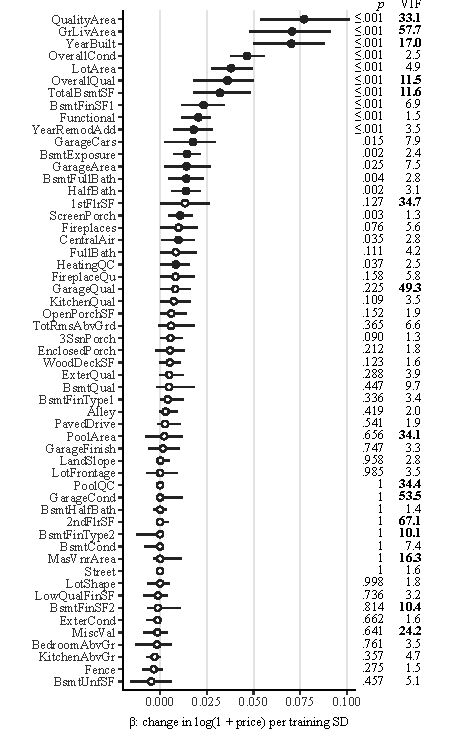
\includegraphics[width=\columnwidth]{figures/coef_forest.pdf}
\caption{All 55 numeric and ordinal coefficients with bootstrap 95\% CIs. Filled: CI excludes 0; $p$: uncorrected bootstrap; bold: VIF $\geq 10$. All 214 columns: \texttt{results/tables/04\_coefficients.md}.}
\label{fig:coef}
\end{figure}

\subsection{Error Analysis}
% Slides p.17 (8%): >= 3 largest-error test cases with actual, predicted, error
% (USD) and context; explain each; shared pattern and the first fix.
% Possible extra pattern (W1 check, discuss with P3/I1 before using): 6 of the 10
% largest errors, incl. all top 3, are SaleCondition = Partial (homes sold before
% completion) vs 9.2% of the test set; sale condition was excluded as a feature.
The three largest test errors (Table~\ref{tab:errors}) are all high-quality homes (OverallQual 8--9) in two of the three most expensive neighborhoods, underpredicted by 17--25\%.
Size alone does not explain this: house 775 is the smallest of the three but has the largest relative error.

The shared pattern: all three were new homes, built one year or less before the sale and sold before completion (sale type ``New'', sale condition ``Partial'').
Four of the ten largest errors are underpredicted new homes of this kind (Ids 899, 775, 1047 and 1244), although homes sold before completion are only 27 of the 292 test sales (9.2\%).
A fifth (Id 582) is overpredicted, so new construction adds error in both directions.
Without the sale year and sale type, the model cannot tell that these houses were brand new when sold.
The quality slices show the same effect: MAE rises from 11{,}085~USD for OverallQual $\leq 5$ to 27{,}636~USD for $\geq 8$ ($n = 45$).
The first fix is better input, not a bigger model: whether a house is newly built can come from building permits or the listing rather than the sale record, so a new-construction flag would respect our pre-sale rule.

\begin{table}[t]
\centering
\small
\setlength{\tabcolsep}{3.5pt}
\begin{tabular}{@{}r r r r l@{}}
\toprule
\textbf{Id} & \textbf{Actual} & \textbf{Pred.} & \textbf{Error} & \textbf{Context} \\
\midrule
899  & 611{,}657 & 473{,}938 & 137{,}719 & Q9, 2{,}364 ft$^2$, NridgHt \\
775  & 395{,}000 & 295{,}840 & 99{,}160  & Q8, 1{,}973 ft$^2$, NridgHt \\
1047 & 556{,}581 & 459{,}516 & 97{,}065  & Q9, 2{,}868 ft$^2$, StoneBr \\
\bottomrule
\end{tabular}
\caption{Largest absolute test errors of the final model (USD; error = actual $-$ predicted, so positive means underprediction). Q: OverallQual; area: GrLivArea.}
\label{tab:errors}
\end{table}
